\documentclass[12pt, aspectratio=169]{beamer}

\usepackage{minted}

\usetheme{metropolis}

\newcommand{\ferrisframe}[1]{%
  \begin{frame}[standout]
    
\includegraphics[height=0.8\textheight]{images/ferris.png}

    #1
  \end{frame}
}

\title{Introduction to Rust}
\date{December 12, 2017}
\author[@aqrln, @nechaido]{%
  \texorpdfstring{%
    \parbox{0.35\textwidth}{%
      Alexey Orlenko\\
      \href{https://twitter.com/aqrln}{@aqrln}
    }
    \parbox{0.35\textwidth}{%
      Dmytro Nechai\\
      \href{https://twitter.com/nechaido}{@nechaido}
    }
    \vspace{0.6cm}
  }
  {Alexey Orlenko, Dmytro Nechai}
}
\institute{HowProgrammingWorks}

\begin{document}

\maketitle

\ferrisframe{Lecture 1}

\begin{frame}{What is Rust}
  \begin{quote}
    ``Rust is a systems programming language that runs blazingly fast, prevents
    segfaults, and guarantees thread safety.''
  \end{quote}

  \rightline{\rm --- \url{https://www.rust-lang.org}}
\end{frame}

\begin{frame}{Rust's main strengths}
  \begin{itemize}
    \item safety
    \item speed
    \item concurrency
  \end{itemize}
\end{frame}

\begin{frame}{Rust's main features}
  \begin{itemize}
    \item Strong static typing with type inference
    \item Trait-based generics
    \onslide<2->{\item Functional programming features}
    \onslide<2->{\item Zero-cost abstractions}
    \onslide<3->{\item Guaranteed memory safety without GC}
    \onslide<3->{\item Threads without data races}
    \onslide<4->{\item Minimal runtime and C ABI}
  \end{itemize}
\end{frame}

\begin{frame}{Who is using Rust}
  \begin{columns}
    \column{0.25\textwidth}
    
\includegraphics[width=\textwidth]{images/mozilla.png}
    \column{0.25\textwidth}
    
\includegraphics[width=\textwidth]{images/dropbox.png}
    \column{0.25\textwidth}
    
\includegraphics[width=\textwidth]{images/atlassian.png}
  \end{columns}

  \begin{columns}
    \column{0.25\textwidth}
    
\includegraphics[width=\textwidth]{images/npm.png}
    \column{0.25\textwidth}
    
\includegraphics[width=\textwidth]{images/bitfury.png}
    \column{0.25\textwidth}
    
\includegraphics[width=\textwidth]{images/sentry.png}
  \end{columns}

  \begin{columns}
    \column{0.25\textwidth}
    
\includegraphics[width=\textwidth]{images/ovh.png}
    \column{0.25\textwidth}
    
\includegraphics[width=\textwidth]{images/coursera.png}
    \column{0.25\textwidth}
    
\includegraphics[width=\textwidth]{images/wire.png}
  \end{columns}
\end{frame}

\begin{frame}{What you can write in Rust}
  \begin{itemize}
    \item Anything you would write in C.
    \item High-performance web servers with \href{https://hyper.rs/}{Hyper}.
    \item Fast algorithms and libraries to use from JavaScript with Asm.js and
      WebAssembly.
  \end{itemize}
\end{frame}

\begin{frame}{Advantages for developers in languages like C or C++}
  \begin{itemize}
    \item Type and memory safety
    \item Zero-cost or low-cost high-level abstractions
    \item Standard tooling and package manager
  \end{itemize}
\end{frame}

\begin{frame}{Advantages for developers in languages like Python or JavaScript}
  \begin{itemize}
    \item Type and memory safety
    \item Performance
    \item Parallelism
    \item Going lower-level without sacrificing expressiveness
  \end{itemize}
\end{frame}

\begin{frame}{Some inspirational links}
  Some inspirational links --- check these out later!

  \begin{itemize}
    \item \url{https://hacks.mozilla.org/2017/08/inside-a-super-fast-css-engine-quantum-css-aka-stylo/}
    \item \url{https://www.youtube.com/watch?v=cNeIOt8ZdAY}
  \end{itemize}
\end{frame}

\begin{frame}{Installing Rust}
  The official tool for managing Rust toolchains and their versions is
  \texttt{rustup}.

  \url{https://rustup.rs}
\end{frame}

\begin{frame}{Rust Flavors}
  \begin{itemize}
    \item \textbf{Stable} --- recommended for most users, unstable features are
      unavailable.
    \item \textbf{Beta} --- preview of the next stable.
    \item \textbf{Nightly} --- latest build from \texttt{master}, unstable
      features are disabled by default, but available through feature-gates.
  \end{itemize}
\end{frame}

\begin{frame}{Managing Rust installation}
  Installing a specific toolchain:

  \texttt{\$ rustup install nightly}

  Updating all toolchains:

  \texttt{\$ rustup update}

  Updating a specific toolchain:

  \texttt{\$ rustup update stable}
\end{frame}

\begin{frame}{Managing Rust installation}
  Adding a new target triple:

  \texttt{\$ rustup target add wasm32-unknown-emscripten}

  \texttt{\$ rustup target add armv7-apple-ios}
\end{frame}

\begin{frame}{Target triples}
  \[\texttt{\{arch\}-\{vendor\}-\{target\}[-\{abi\}]}\]
\end{frame}

\begin{frame}{Built-in tools}
  \begin{itemize}
    \item \texttt{rustc} --- the Rust compiler
    \item \texttt{rustdoc} --- documentation generator
    \item \texttt{cargo} --- project management tool
    \item \texttt{rust-lldb}, \texttt{rust-gdb} --- wrappers for \texttt{lldb}
      and \texttt{gdb} debuggers
  \end{itemize}
\end{frame}

\begin{frame}{Cargo}
  Cargo is Rust's package manager, build system and overall project management
  tool.

  \begin{columns}
    \begin{column}{0.3\textwidth}
      \begin{itemize}
        \item \texttt{cargo new}
        \item \texttt{cargo run}
        \item \texttt{cargo build}
        \item \texttt{cargo check}
      \end{itemize}
    \end{column}

    \begin{column}{0.5\textwidth}
      \begin{itemize}
        \item \texttt{cargo test}
        \item \texttt{cargo bench}
        \item \texttt{cargo doc}
        \item \texttt{cargo install}
      \end{itemize}
    \end{column}
  \end{columns}
\end{frame}

\begin{frame}{crates.io}
  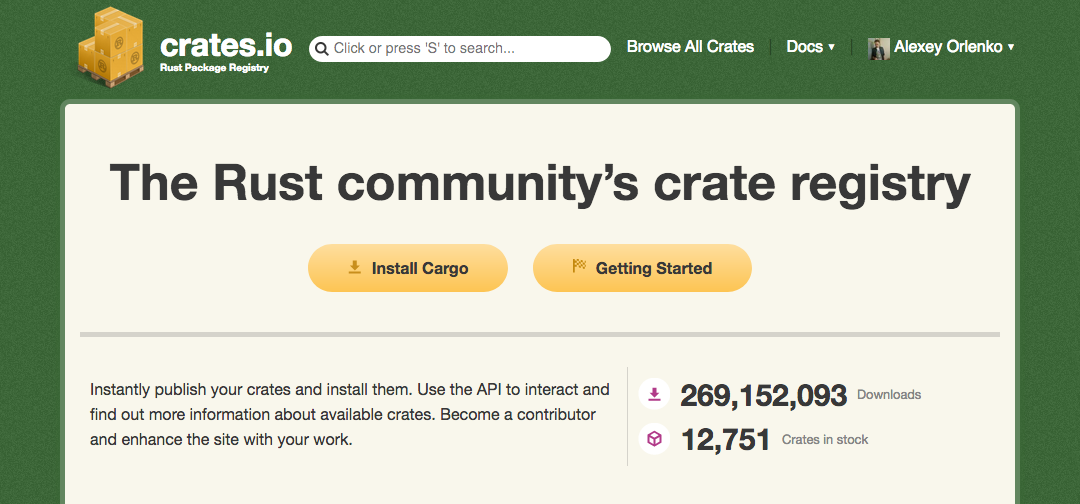
\includegraphics[width=\textwidth]{images/crates-io.png}
\end{frame}

\begin{frame}{docs.rs}
  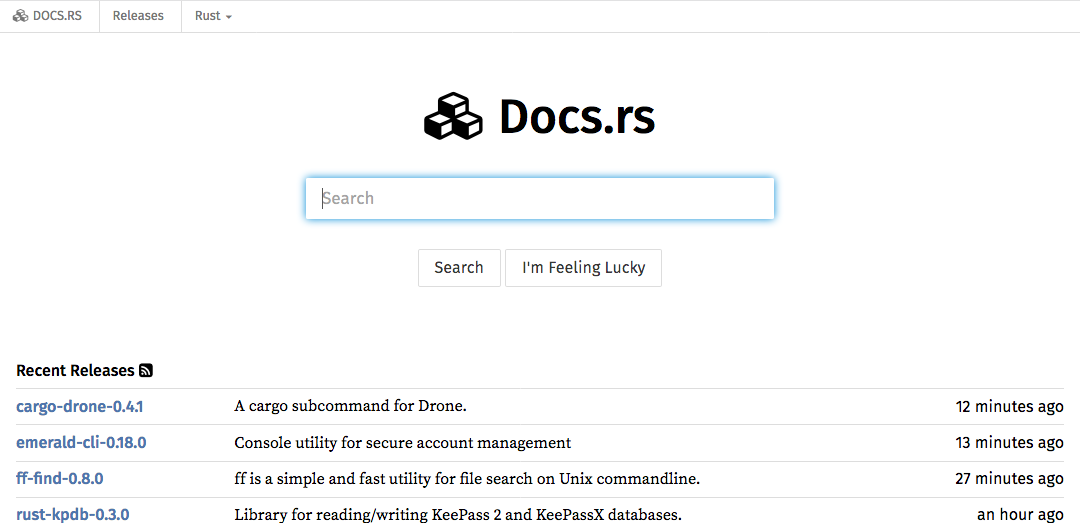
\includegraphics[width=\textwidth]{images/docs-rs.png}
\end{frame}

\begin{frame}{Rustfmt}
  Rustfmt formats your code according to the
  \href{https://github.com/rust-lang-nursery/fmt-rfcs}{official styleguide}.

  Installing:

  \texttt{\$ cargo install rustfmt}

  or

  \texttt{\$ cargo +nightly install rustfmt-nightly}

  Formatting all sources in the project:

  \texttt{\$ cargo fmt}
\end{frame}

\begin{frame}{Clippy}
  Rust compiler includes a basic built-in linter. \texttt{clippy} is a compiler
  plugin that adds \textbf{208} additional advanced lints to catch common
  mistakes and help you write idiomatic code.

  \texttt{\$ cargo +nightly install clippy}

  \texttt{\$ cargo clippy}
\end{frame}

\begin{frame}{Useful external cargo subcommands}
  Improved dependency management:

  \texttt{\$ cargo install cargo-edit}

  Usage:

  \texttt{\$ cargo add crate-name}

  \texttt{\$ cargo rm crate-name}

  \texttt{\$ cargo upgrade}
\end{frame}

\begin{frame}{Useful external cargo subcommands}
  Updating globally installed binary crates:

  \texttt{\$ cargo install cargo-update}

  Usage:

  \texttt{\$ cargo install-update crate-name}

  \texttt{\$ cargo install-update -a}
\end{frame}

\begin{frame}{Useful external cargo subcommands}
  Watching the project and running a command (\texttt{cargo check} by default)
  automatically:

  \texttt{\$ cargo install cargo-watch}

  Usage:

  \texttt{\$ cargo watch}

  \texttt{\$ cargo watch -x test}
\end{frame}

\begin{frame}{Installing something else useful with cargo, while we are here}
  \texttt{ack} is better than \texttt{grep}, and \texttt{ag} is faster than
  \texttt{ack}, right? It's not fast enough compared to \texttt{rg}.

  \texttt{\$ cargo install ripgrep}

  By the way, Visual Studio Code comes bundled with \texttt{ripgrep} as its
  search backend, so if you use VS Code, you have probably used \texttt{rg}
  without even realizing it.
\end{frame}

\begin{frame}{Plugins for editors}
  \begin{itemize}
    \item Vim: \url{https://github.com/rust-lang/rust.vim}
    \item Emacs: \url{https://github.com/rust-lang/rust-mode}
    \item VS Code: \url{https://marketplace.visualstudio.com/items?itemName=rust-lang.rust}
    \item IntelliJ IDEA: \url{https://intellij-rust.github.io}
  \end{itemize}
\end{frame}

\begin{frame}{Useful services}
  \begin{itemize}
    \item \url{https://play.rust-lang.org/} --- Rust Playground. Pastebin for
      snippets of Rust code you can run right in your browser and share with
      others (e.g., in a chat when you need some help).
    \item \url{https://rust.godbolt.org/} --- Compiler Explorer. Another
      pastebin-like service integrated with the compiler. Instead of running
      the code, it only compiles it and shows the correspondence between Rust
      and Assembly code.
  \end{itemize}
\end{frame}

\begin{frame}{Resources for learning Rust}
  \begin{itemize}
    \item Rust Book \only<2>{---\\
      \url{https://doc.rust-lang.org/book/}}
    \item Rustonomicon \only<3>{---\\ \url{https://doc.rust-lang.org/nomicon/}}
    \item Unstable Book \only<4>{---\\
      \url{https://doc.rust-lang.org/beta/unstable-book/}}
    \item Reference \only<5>{---\\ \url{https://doc.rust-lang.org/reference/}}
  \end{itemize}
\end{frame}

\begin{frame}{Links}
  This presentation: \url{https://github.com/HowProgrammingWorks/rust-meetups}

  Telegram chat: \url{https://t.me/HowProgrammingWorks}
\end{frame}

\ferrisframe{Code}

\begin{frame}[fragile]{Hello World}
  \begin{minted}{rust}
  fn main() {
    println!("Hello!");
  }
  \end{minted}
\end{frame}

\begin{frame}[fragile]{Declaring variables}
  \begin{minted}{rust}
    let integer = 1;
    let unsigned: u8 = 1;
    let mut mutable_integer = 2;

    integer = 1; // Error here
    mutable_integer = 3;
  \end{minted}
\end{frame}

\begin{frame}[fragile]{Conditions}
  \begin{minted}{rust}
    let x = 5;

    if x == 5 {
        println!("x is five!");
    } else {
        println!("x is not five :(");
    }

    let y = if x == 5 { 10 } else { 15 };
  \end{minted}
\end{frame}

\begin{frame}[fragile]{Loops: loop}
  \begin{minted}{rust}
    loop {
        println!("Loop forever!");
        break;
    }
  \end{minted}
\end{frame}

\begin{frame}[fragile]{Loops: while}
  \begin{minted}{rust}
    let mut x = 5;
    let mut done = false;

    while !done {
        x += x - 3;

        println!("{}", x);

        if x % 5 == 0 {
            done = true;
        }
    }
  \end{minted}
\end{frame}

\begin{frame}[fragile]{Loops: for}
  \begin{minted}{rust}
    for x in 0..10 {
        println!("{}", x);
    }

    for x in (0..10).rev() {
        println!("{}", x);
    }
  \end{minted}
\end{frame}

\begin{frame}[fragile]{Matching}
  \begin{minted}{rust}
    let x = 5;

    match x {
        1 => println!("one"),
        2 => println!("two"),
        3 => println!("three"),
        4 => println!("four"),
        5 => println!("five"),
        _ => println!("something else"),
    }
  \end{minted}
\end{frame}

\begin{frame}[fragile]{Matching: getting a value}
  \begin{minted}{rust}
    let x = 5;

    let number = match x {
        1 => "one",
        2 => "two",
        3 => "three",
        4 => "four",
        5 => "five",
        _ => "something else",
    };
  \end{minted}
\end{frame}

\begin{frame}[fragile]{Matching: multiple patterns}
  \begin{minted}{rust}
    let x = 1;

    match x {
        1 | 2 => println!("one or two"),
        3 => println!("three"),
        _ => println!("anything"),
    }
  \end{minted}
\end{frame}

\begin{frame}[fragile]{Matching: matching a range}
  \begin{minted}{rust}
    let x = 1;

    match x {
        1 ... 5 => println!("one through five"),
        _ => println!("anything"),
    }
  \end{minted}
\end{frame}

\begin{frame}[fragile]{Matching: binding}
  \begin{minted}{rust}
    let x = 1;

    match x {
        e @ 1 ... 5 => println!("{}", e),
        _ => println!("anything"),
    }
  \end{minted}
\end{frame}

\begin{frame}[fragile]{Matching: guards}
  \begin{minted}{rust}
    let x = 4;
    let y = false;

    match x {
        4 | 5 if y => println!("yes"),
        _ => println!("no"),
    }
  \end{minted}
\end{frame}

\ferrisframe{Thanks for coming and see you next time!}

\end{document}
